\documentclass{article}
\usepackage[a4paper,width=170mm,top=30mm,bottom=30mm]{geometry}
\usepackage[utf8]{inputenc}
\usepackage[T1]{fontenc}
\usepackage[portuguese]{babel}
\usepackage{hyphenat}
\hyphenation{mate-mática recu-perar}
\usepackage{graphicx}
\usepackage{caption}
\usepackage{subcaption}
\usepackage{color}

\title{
{\huge Laboratório de Física}\\{\Large Relatório 1}}
\author{Fabio DESTRO 10284667\\Vitor TORRES 10284952\\}
%\date{07 Março 2018}
\date{\today}

\begin{document}

\begin{figure}[t]
    \begin{subfigure}{0.49\textwidth}
        \centering
        
\includegraphics[width=0.8\textwidth]{brasao_usp_pb.png}
    \end{subfigure}
    \hfill
    \begin{subfigure}{0.49\textwidth}
       \centering
        
\includegraphics[width=0.8\textwidth]{LOGO_ICMC_RGB.png}
    \end{subfigure}
\end{figure}

\begin{titlepage}
\centering
{\Large
{\color{white}.\\.\\.} \\
Universidade de São Paulo\\
Instituto de Ciências Matemáticas e de Computação\\\vspace{1.8mm}
Instituto de Física de São Carlos}
\vfill
Prática 1:\\
{\Large
Medidas de grandezas físicas}
\vfill
Alunos
\begin{tabular}{c c}
    Fabio F. Destro & 10284667\\
    Vitor G. Torres & 10284952
\end{tabular}
\vfill
Docente
\begin{tabular}{c c}
    Osvaldo N. O. Junior
\end{tabular}
\vfill
São Carlos, \today\\
\end{titlepage}
%\maketitle
\newpage

%\tableofcontents
%\newpage

\begin{abstract}
\indent
Contextualização:

A intenção desta primeira aula prática foi nos familiarizar com conceitos de medidas de grandezas físicas e suas incertezas, levando-nos a trabalhar cálculos com precisão de instrumentos e propagação de erros.

Proposito:

E com esses calculos entender 

Metodologia:



Principais resultados:



Conclusao:



\end{abstract}
\newpage

\section{Introdução}
\indent
sngjntsrn
\section{Metodologia}
\subsection{Primeiro Procedimento}
\indent

Para calcularmos o volume do sólido percorremos dois caminhos distintos, o direto e o indireto:

Diretamente: Utilizando uma proveta graduada (precisão de $0.5mm$), com água, aferimos o volume inicial da água, em seguida colocamos o sólido em seu interior e a partir da diferença, temos o volume do sólido.

Indiretamente: Com o auxílio do paquímetro (precisão de $0.05mm$) medimos cada dimensão necessária para o cálculo de seu volume $V = \pi R^2 h$. Sendo que seu volume é determinado pelo volume de um cilindro grande com a subtração de um menor, como indicado na figura 1.

\begin{figure}[h]
    \centering
    %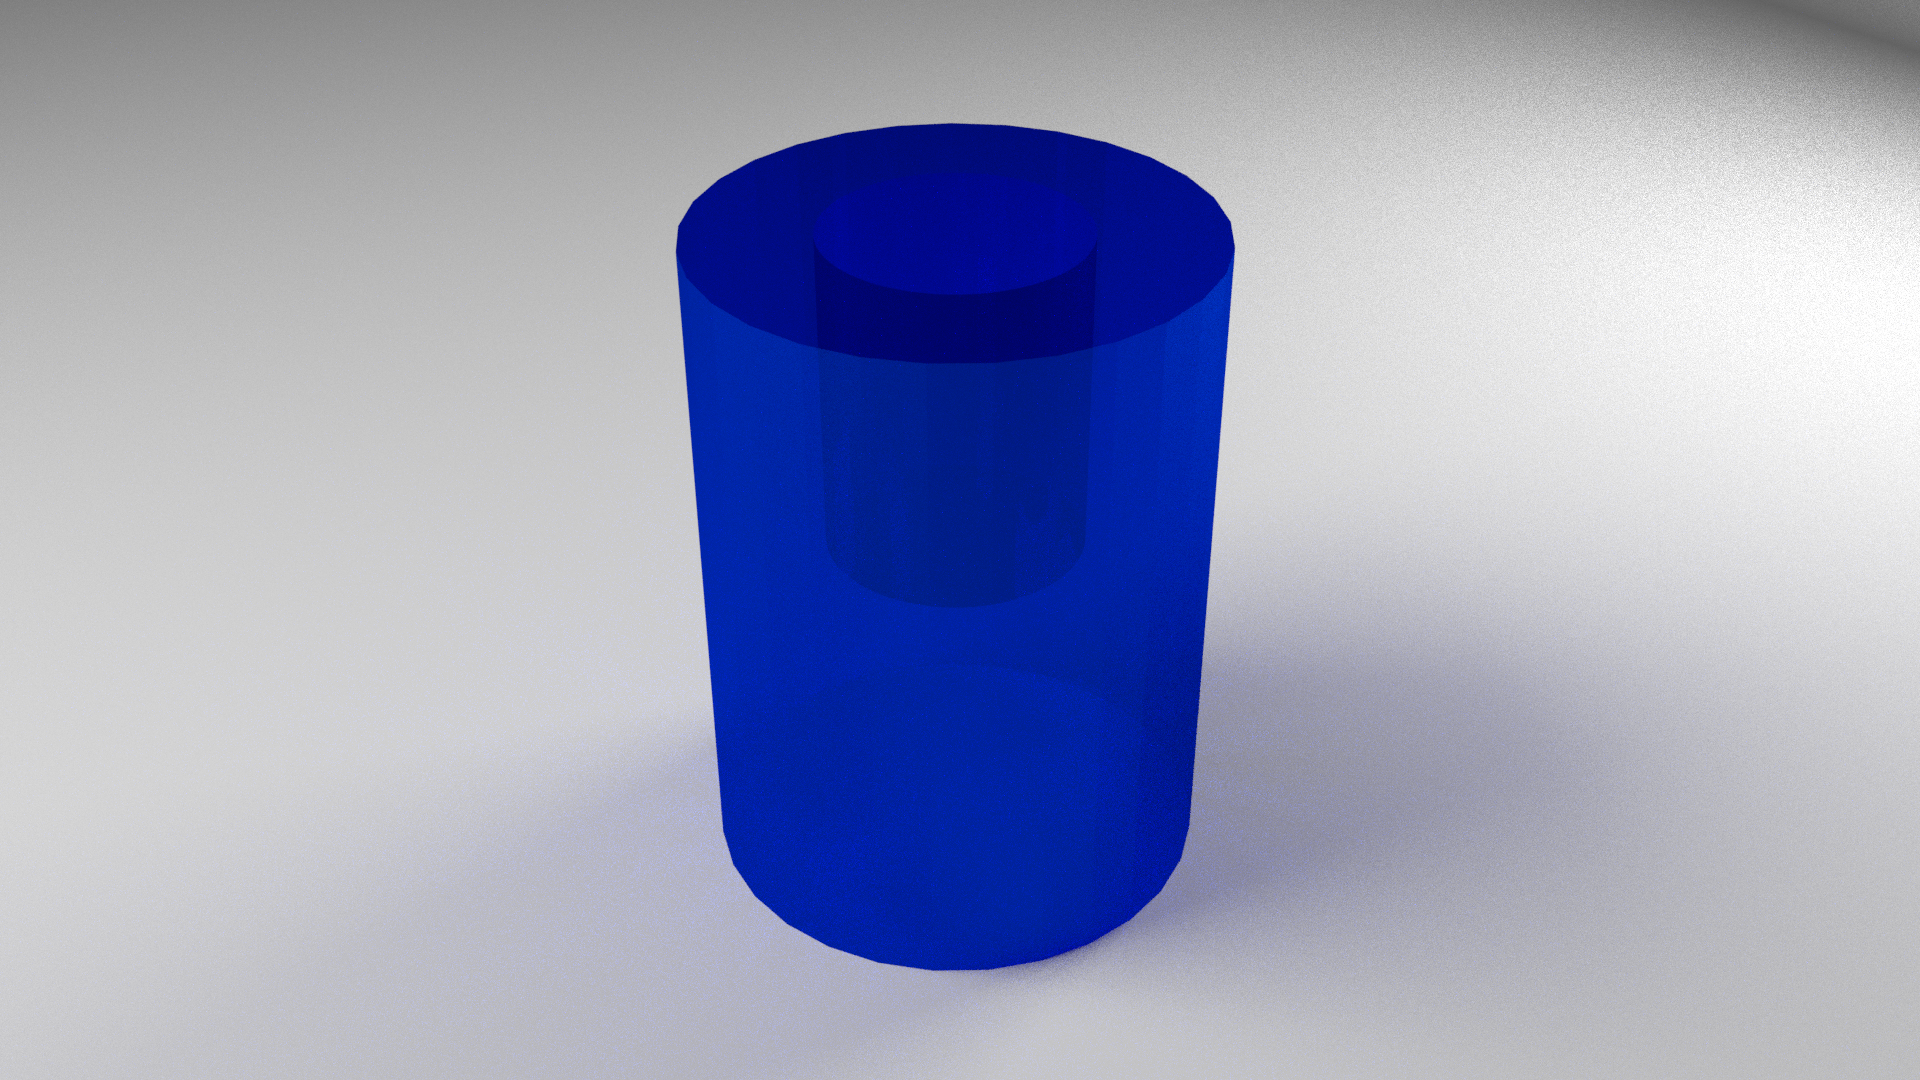
\includegraphics[scale=0.1]{a0002.png}
    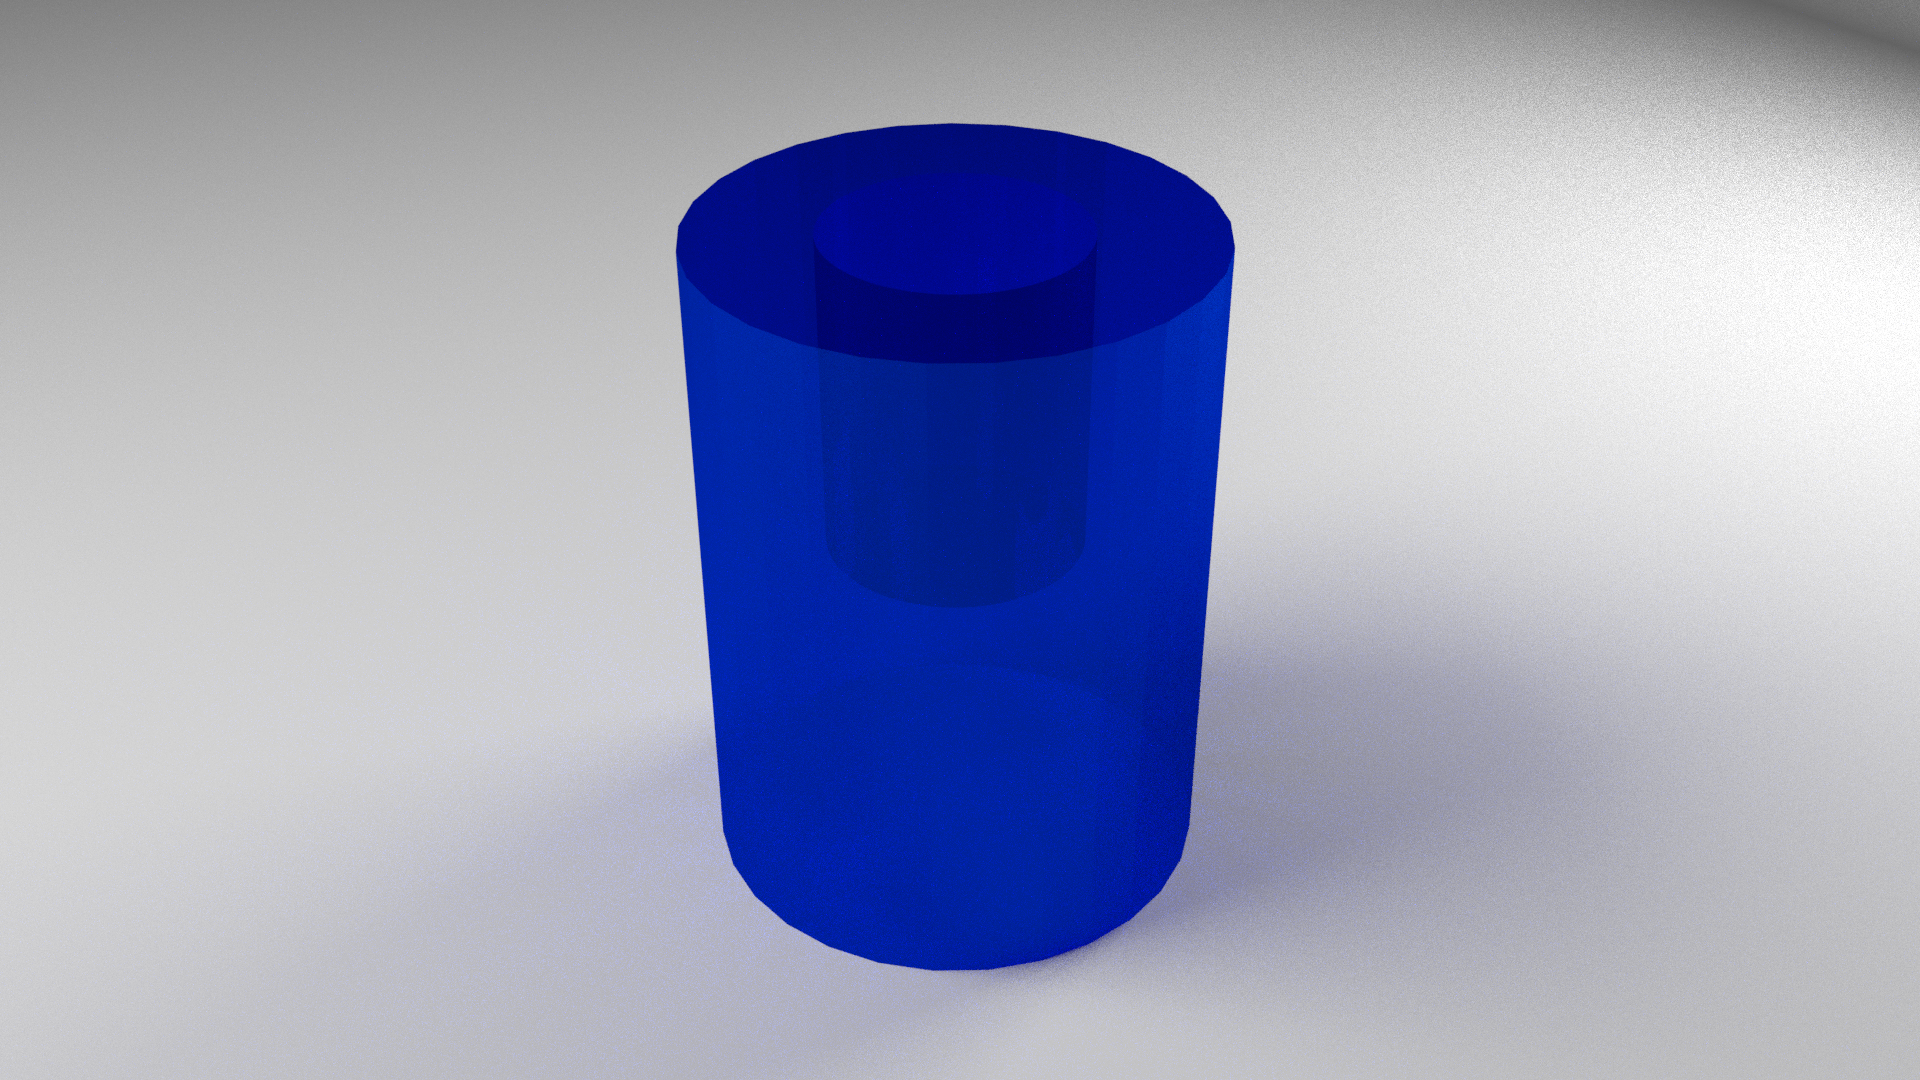
\includegraphics[width=0.5\textwidth]{a0002.png}
    \caption{Representação do sólido a ser estudado}
    \label{fig:solido}
\end{figure}


\subsubsection{Volume Direto do Cilindro}
Dados:

$V_I = 77\;mm\; =$ volume inicial da proveta;

$V_F = 91\;mm\; =$ volume final da proveta;

$\sigma_{V_F} = \sigma_{V_I} = 0.5\;mm\;=$ precisão da proveta.

\[V = V_F - V_I\]
\[V = (91 \pm \sigma_{V_F})-(77 \pm \sigma_{V_I})\]
\[V = 91-77\pm\sigma_{V}\]
\[V= (14 \pm\sigma_{V})\; cm^3\]
\[\sigma_{V}^2 = \left(\frac{dV}{dV_F}\right)^2\sigma_{V_F}^2+\left(\frac{dV}{dV_I}\right)^2\sigma_{V_I}^2\]
\[\sigma_{V} = \pm\sqrt{1^2\cdot0.5^2+1^2\cdot0.5^2}=\pm0.707106781187\]
\[V= (14 \pm0.71)\; cm^3\]


\subsubsection{Volume Indireto do Cilindro}
Dados:

$H = 41.05\;mm\;=$ altura do cilindro maior (externo);

$D = 22.1\;mm\;=$ diâmetro do cilindro maior;

$h = 18.85\;mm\;=$ altura do cilindro menor (interno);

$d = 12\;mm\;=$ diâmetro do cilindro menor;

$\sigma_H = \sigma_D = \sigma_h = \sigma_d = 0.05\;mm\;=$ precisão do paquímetro.

\[V = \pi \left(\left(\frac{D}{2}\right)^2\cdot H-\left(\frac{d}{2}\right)^2\cdot h\right)\]
\[V = \pi \left(\left(\frac{22.1\pm0.05}{2}\right)^2\cdot \left(41.05\pm0.05\right)-\left(\frac{12\pm0.05}{2}\right)^2\cdot \left(18.85\pm0.05\right)\right)\]
\[V = \pi \left(\left(\frac{22.1}{2}\right)^2\cdot 41.05-\left(\frac{12}{2}\right)^2\cdot 18.85\right)+\sigma_V\]
\[V = 13614.74403750607\pm\sigma_V\]
\vline
\[\sigma_V^2=\left(\frac{dV}{dD}\right)^2\sigma_D^2+\left(\frac{dV}{dH}\right)^2\sigma_H^2+\left(\frac{dV}{dd}\right)^2\sigma_d^2+\left(\frac{dV}{dh}\right)^2\sigma_h^2\]
\[\sigma_V^2=\left(\left(\frac{2\pi DH}{4}\right)^2+\left(\frac{\pi D^2}{4}\right)^2+\left(-\frac{2\pi dh}{4}\right)^2+\left(-\frac{\pi d^2}{4}\right)^2\right)\cdot0.0025\]
\[\sigma_V^2=\left(4D^2H^2+D^4+4d^2h^2+d^4\right)\cdot\frac{0.0025\pi^2}{16}\]
\[\sigma_V=\pm\sqrt{\left(4\left(22.1\right)^2\left(41.05\right)^2+\left(22.1\right)^4+4\left(12\right)^2\left(18.85\right)^2+\left(12\right)^4\right)\cdot\frac{0.0025\pi^2}{16}}\]
\[\sigma_V=\pm76.10696380652162\:mm^3\]
\[V = (13.61474403750607\pm0.07610696380652162)\:cm^3\]
\[V = (13.61\pm0.08)\:cm^3\]

Comparando o resultado do cálculo direto e indireto do volume do sólido, é possível perceber que os valores encontrados em ambos os métodos são condizentes e estão coerentes, uma vez que os volumes estão próximos e dentro do limite de erro. Além disso, foi possível observar que o método indireto foi mais preciso, uma vez que possui um erro menor, em relação ao método direto.

Isso ocorre já que as medidas obtidas pelo método indireto ocorreram utilizando um instrumento com maior precisão (paquímetro) em relação à proveta graduada mesmo com a propagação de erro para o cálculo do volume indireto.


\subsection{Segundo Procedimento}
Dados:

$M = 36.74\;g\; = $ massa do sólido

$\sigma_M = 0.01\;g\; = $ precisão da balança

\[\rho = \frac{M\;(g)}{V\;(cm^3)} = \frac{(36.74\pm0.01)}{(13.61474403750607\pm0.07610696380652162)}\]
\[\rho = 2.698545040493467 \pm \sigma_\rho\]
\[\sigma_\rho^2 = \left(\frac{d\rho}{dM}\right)^2\sigma_M^2+\left(\frac{d\rho}{dV}\right)^2\sigma_V^2\]
%\[\sigma_\rho = \sqrt{\left(\frac{1}{M}\right)^2 0.01 + \left(-\frac{M}{V^2}\right)^2 0.07610696380652162}\]
\[\sigma_\rho =\pm 0.015102845745\]
\[\rho = (2.70 \pm 0.02)\;g/cm^3\]

A partir do cálculo da densidade e com o auxílio de uma tabela com a densidade de diversos materiais foi possível concluir que o material do sólido é o alumínio, já que sua densidade é correspondente já que o alumínio na tabela de referência apresenta valor $2.699\;(g/cm^3)$. Com esses dados, comparando grandezas fisicas com incertezas, utilizando $|x_1-x_2|<2(\sigma_1+\sigma_2)$ foi possível perceber que são equivalentes.

\subsection{Terceiro Procedimento}

\begin{table}[!ht]
    \centering
    \begin{tabular}{c|c}
        $d\;(mm)$ & $|d_i-\bar{d}|\;(mm)$ \\\hline
        2.83 & 0.06200\\
        2.76 & 0.00800\\
        2.96 & 0.15200\\
        2.73 & 0.03800\\
        2.69 & 0.07800\\
        2.76 & 0.00800\\
        2.83 & 0.06200\\
        2.72 & 0.04800\\
        2.71 & 0.05800\\
        2.73 & 0.03800\\
    \end{tabular}
    \caption{Medidas aferidas e o desvio do padrão}
    \label{tab:my_label}
\end{table}
\[\sum_{i=0}^N \frac{|d_i-\bar{d}|}{N}=\sum_{i=0}^{10} \frac{|d_i-2.768|}{10}=0.0552\]
\indent
Além disso, no cálculo da média entre os diâmetro, fazendo a propagação de erros, é possível encontrar: $\bar{d} = (2.768 \pm 0.01)\;mm$.

Como o desvio padrão foi maior que o erro propagado, deve ser usado o desvio padrão como margem de erro, portanto: $\bar{d} = (2.768 \pm 0.0552)\;mm = (2.77 \pm 0.05)\;mm$

A diferença entre medir o diametro sempre no mesmo ponto ou em pontos diferentes é levar em consideração a variação da forma do objeto.

\section{Resultados e discussão}
\end{document}
